%%
% La siguiente plantilla esta basada en el siguiente enlace:
% http://academic.reed.edu/physics/courses/Physics332.s08/reports.html
% La plantilla original puede descargarse de ese sitio
% Se dejo parte del texto original en inglés para ilustar el uso de la plantilla
% Se hicieron algunas modificaciones para ajustar el idioma y otros detalles para 
% completar un reporte técnico breve pero muy puntual
% Modificación Inicial: Marco Aurelio Nuno Maganda - 11/SEP/2014
% 
% Enlace a la documentación del tipo de documento base (revtex4)
% http://mirror.hmc.edu/ctan/macros/latex/contrib/revtex/doc/latex/revtex/source/revtex4-1.pdf
%
% En algunas distribuciones es necesario instalar el paquete texlive-publishers
%
%\documentclass[letterpaper,aps,twocolumn,pre,nofootinbib]{revtex4}
%\documentclass[twocolumn]{article}
\documentclass[conference]{IEEEtran}

\usepackage[spanish]{babel}
\usepackage{amsmath,amssymb,amsfonts,amsthm}
\usepackage{graphicx}
%\usepackage{bbm}
\usepackage[utf8]{inputenc} % Caracteres en Español (Acentos, ñs)
\usepackage{url} % ACENTOS
\usepackage{hyperref} % Referencias
\usepackage{subfig}
\usepackage{lipsum}
\usepackage{balance}
\usepackage{listings}
\usepackage{xcolor}
\usepackage{float}

\lstset{
    basicstyle=\ttfamily\small,  % Aquí puedes cambiar a \footnotesize o \scriptsize
    keywordstyle=\color{blue}\bfseries,
    commentstyle=\color{gray},
    stringstyle=\color{orange},
    showstringspaces=false,
    numberstyle=\tiny\color{gray},
    numbers=left,
    stepnumber=1,
    numbersep=10pt,
    frame=single,
    backgroundcolor=\color{lightgray!20},
    captionpos=b,
    breaklines=true,
    breakatwhitespace=true,
    tabsize=4,
    language=Python
}


%%%%%%%%%%%%%%%%%%%%%%%%%%%%%%%%%%%%%%%%%%%%%
% PARCHE PARA ELIMINAR LA FECHA DEL DOCUMENTO
% 
\usepackage{etoolbox}
\makeatletter
% \frontmatter@RRAP@format is responsible for the parentheses
\patchcmd{\frontmatter@RRAP@format}{(}{}{}{}
\patchcmd{\frontmatter@RRAP@format}{)}{}{}{}
%\renewcommand\Dated@name{}
\makeatother	
% FIN DEL PARCHE
% 
%%%%%%%%%%%%%%%%%%%%%%%%%%%%%%%%%%%%%%%%%%%%%

%%%%%%%%%%%%%%%%%%%%%%%%%%%%%%%%%%%%%%%%%%%%%
% PARCHE PARA PERMIRIR UTILIZAR BIBLATEX EN ESTA PANTLLA
%\PassOptionsToPackage{square,numbers}{natbib}
%\RequirePackage{natbib}  
%%%%%%%%%%%%%%%%%%%%%%%%%%%%%%%%%%%%%%%%%%%%%

\usepackage[backend=bibtex,sorting=none]{biblatex}
% Estas lineas permiten romper los hipervinculos muy largos !!!!
\setcounter{biburllcpenalty}{7000}
\setcounter{biburlucpenalty}{8000}
\addbibresource{references.bib}

% Actualiza en automático la fecha de las citas de internet a la fecha de la compilación del documento
\usepackage{datetime}
\newdateformat{specialdate}{\twodigit{\THEDAY}-\twodigit{\THEMONTH}-\THEYEAR}
\date{\specialdate\today}

% la sentencia \burl en las citas... 
\usepackage[hyphenbreaks]{breakurl}

\renewcommand\spanishtablename{Tabla}
\renewcommand\spanishfigurename{Figura}

%\usepackage{datetime}
%\newdateformat{specialdate}{\twodigit{\THEDAY}-\twodigit{\THEMONTH}-\THEYEAR}
%\newdateformat{specialdate}{\twodigit{\THEDAY}-\THEYEAR}
%\date{\specialdate\today}


\begin{document}
%%%%%%%%%%%%%%%%%%%%%%%%%%%%%%%%%%%%%%%%%%%%%
% Definitions
%
%
% Define your special symbols here
%
%%%%%%%%%%%%%%%%%%%%%%%%%%%%%%%%%%%%%%%%%%%%%

% use to set width of figures
\newcommand{\breite}{0.9} %  for twocolumn
\newcommand{\RelacionFiguradoscolumnas}{0.9}
\newcommand{\RelacionFiguradoscolumnasPuntoCinco}{0.45}


%%%%%%%%%%%%%%%%%%%%%%%%%%%%%%%%%%%%%%%%%%%%%
% End Definitions
%%%%%%%%%%%%%%%%%%%%%%%%%%%%%%%%%%%%%%%%%%%%%


%Title of paper
\title{Reporte de Proyecto en Equipo 04 de Unidad III \\ Recorrido virtual UPV}

% Trabajo Individual
\author{\IEEEauthorblockN{González Cortés Israel Guadalupe\IEEEauthorrefmark{1}, Guzmán González Daniel Alejandro\IEEEauthorrefmark{1}, 
Peña Cuéllar Aldo de Jesús\IEEEauthorrefmark{1}, \\ Pérez Facundo Adrián\IEEEauthorrefmark{1}, 
Treviño Gandarilla Jesús David\IEEEauthorrefmark{1}}
% En caso de trabajos en equipo, poner a todos los autores en estricto ORDEN ALFABETICO
%\author{\IEEEauthorblockN{Michael Shell\IEEEauthorrefmark{1},
%Homer Simpson\IEEEauthorrefmark{1},
%James Kirk\IEEEauthorrefmark{1}, 
%Montgomery Scott\IEEEauthorrefmark{1} and
%Eldon Tyrell\IEEEauthorrefmark{1}}
\IEEEauthorblockA{\IEEEauthorrefmark{1}Ingeniería en Tecnologías de la Información\\
Universidad Politécnica de Victoria}
}


%\date{}

\maketitle

\begin{abstract} 
El proyecto de recorrido virtual de la Universidad Politécnica de Victoria, tiene como objetivo implementar una experiencia de realidad virtual para explorar las instalaciones de la universidad. Esta aplicación móvil permite a los usuarios conocer las instalaciones y obtener una representación visual sin necesidad de asistir físicamente. Ofrece una solución interactiva que facilita tanto a estudiantes como visitantes una visión inmersiva y detallada de los espacios del campus.
\end{abstract}


%\maketitle must follow title, authors, abstract, \pacs, and \keywords




\section{Introducción}
El presente informe detalla el proceso de desarrollo de una aplicación móvil diseñada para ofrecer un recorrido virtual \cite{Sh:1} de las instalaciones de la Universidad Politécnica de Victoria. Este proyecto surge como una solución innovadora que emplea tecnologías de realidad virtual para proporcionar una experiencia inmersiva y accesible, permitiendo a los usuarios explorar el campus sin necesidad de una visita física.

La aplicación permite la visualización del campus universitario mediante dispositivos móviles y, opcionalmente, cascos de realidad virtual para una mayor inmersión. Para mejorar la interacción con el entorno virtual, se incorporó el uso de controles compatibles, como un mando de Xbox con conectividad Bluetooth \cite{Sh:5}, optimizando la experiencia del usuario al ofrecer una navegación intuitiva y eficiente.

A lo largo del informe, se abordarán las decisiones técnicas, los retos enfrentados y las tecnologías utilizadas para garantizar un diseño funcional e interactivo. El objetivo principal del proyecto es facilitar el acceso remoto a la universidad mediante una herramienta moderna, que promueva tanto la innovación tecnológica como una experiencia de usuario inmersiva.
 
 
\section{Desarrollo Experimental}

En el presente trabajo, se desarrolló una aplicación móvil que permite realizar un recorrido virtual de la Universidad Politécnica de Victoria, integrando tecnologías de realidad virtual y gráficos en 3D \cite{Sh:7}. Para lograrlo, se empleó OpenGL \cite{Sh:2} para la generación y manipulación de texturas, siguiendo el pipeline gráfico correspondiente. Adicionalmente, se utilizó el Cardboard SDK \cite{Sh:6} para implementar la vista en estereoscopio y habilitar el movimiento de cámara en 360°, proporcionando una experiencia inmersiva al usuario.

El recorrido virtual original fue tomado como base, incorporando funcionalidades como el desplazamiento de la cámara y la configuración del mando Xbox. El control Bluetooth se configuró para facilitar la interacción, permitiendo al usuario navegar por el recorrido y reiniciarlo mediante el botón "A" del mando. Este enfoque asegura una experiencia intuitiva y accesible, tanto para usuarios expertos como novatos.

Una parte crítica del desarrollo consistió en integrar las texturas y shaders mediante OpenGL \cite{Sh:3}, ajustando la matriz Model View Projection (MVP) \cite{Sh:9} con los valores generados por el Cardboard SDK \cite{Sh:8}. Este ajuste fue esencial para lograr una proyección precisa de las texturas en el entorno virtual. Además, se agregó el logo de la universidad como un elemento visual distintivo, reforzando la identidad institucional en la aplicación.

Se realizaron pruebas exhaustivas para garantizar la funcionalidad del recorrido, asegurando que las texturas se proyectaran correctamente y que el movimiento de la cámara ofreciera una experiencia fluida y sin interrupciones. Estas pruebas también incluyeron la validación del reinicio del recorrido y la correcta respuesta de los controles del mando Xbox.

El objetivo principal fue ofrecer a los usuarios una herramienta que les permita explorar las instalaciones de la Universidad Politécnica de Victoria de manera virtual. Esto facilita que personas de otras entidades o futuros estudiantes conozcan los diferentes edificios del campus, fomentando un acceso inclusivo e innovador. El desarrollo final resultó en una aplicación eficiente y versátil, capaz de proporcionar una experiencia inmersiva y accesible a diversos perfiles de usuarios.

La clase CubeRenderer es responsable de renderizar un entorno 3D en una aplicación de realidad virtual utilizando OpenGL ES 2.0. Se ocupa de gestionar la cámara, los objetos, las texturas y las transformaciones necesarias para mostrar un espacio virtual interactivo.


La clase MainActivity es el punto de entrada principal de una aplicación de realidad virtual basada en Android, utilizando herramientas como OpenGL ES y la biblioteca Cardboard para renderizar gráficos en 3D. Hereda de CardboardActivity e implementa la interfaz CardboardView.StereoRenderer, lo que permite aprovechar capacidades de renderización estéreo y controlar elementos visuales en un entorno de realidad virtual. Su estructura está diseñada para manejar diferentes aspectos de una escena 3D, como la representación de un cubo, un triángulo y un piso, además de permitir la interacción del usuario mediante dispositivos de entrada como joysticks y el D-Pad.

En términos de diseño de la escena, esta clase utiliza coordenadas y colores definidos previamente para los elementos que se renderizarán, como el cubo, el triángulo y el piso. Además, emplea transformaciones de matrices para posicionar, rotar y escalar estos objetos en el espacio 3D. Por ejemplo, el cubo tiene una distancia inicial definida de 5 unidades y una rotación aplicada en los ejes X e Y, mientras que el triángulo y el piso se posicionan en ubicaciones específicas de la escena. Estas transformaciones se gestionan mediante matrices como modelViewProjection y lightPosInEyeSpace, que también se usan para calcular las posiciones relativas de los elementos y la iluminación.

La clase también integra un sistema de interacción que utiliza el Dpad y entradas de joystick para mover los objetos de la escena. Por ejemplo, el D-Pad permite al usuario desplazar el cubo hacia adelante, atrás, izquierda o derecha, mientras que las entradas del joystick se usan para ajustar su posición o rotación. Estos eventos se procesan en los métodos onGenericMotionEvent y processJoystickInput, donde se extraen las coordenadas de los movimientos y se aplican transformaciones a los objetos correspondientes.

En cuanto a la renderización, la clase implementa métodos para inicializar, compilar y usar shaders de OpenGL ES que controlan cómo se renderizan los objetos en la escena. Los métodos drawTriangle, drawCube y drawFloor se encargan de renderizar cada elemento utilizando programas de sombreado específicos, configurando atributos como posiciones, colores, y normales de los vértices, además de aplicar las matrices de transformación. También se incluyen buffers de datos para los vértices, colores y normales, que se cargan en memoria y se configuran para ser utilizados por los shaders durante la renderización.

Finalmente, MainActivity configura los eventos principales de la aplicación, como la creación de la superficie de renderización y el manejo de cada cuadro renderizado. Durante la inicialización, el método onSurfaceCreated prepara la escena y compila los shaders necesarios, mientras que onDrawEye se encarga de renderizar los elementos según la vista proporcionada por cada ojo en el entorno de realidad virtual. Además, el método onNewFrame actualiza la vista de la cámara y procesa transformaciones basadas en los movimientos del usuario, como rotaciones de cabeza capturadas mediante HeadTransform. Esta implementación permite crear una experiencia interactiva e inmersiva en un entorno de realidad virtual.


\section{Resultados}
A continuación, se presentarán diversas figuras que demostrarán 
los resultados obtenidos en el desarrollo de la aplicación en cuestión. Además, se proporcionará una explicación lo más detallada y completa posible de cada una de ellas, dando a entender sus respectivas funcionalidades.


En la figura \ref{fig:e1}, Se muestra la entrada de la UPV dentro del recorrido virtual, así como la interfaz de la aplicación diseñada para ser compatible con cascos de realidad virtual.

\begin{figure}[h]
    \centering
        {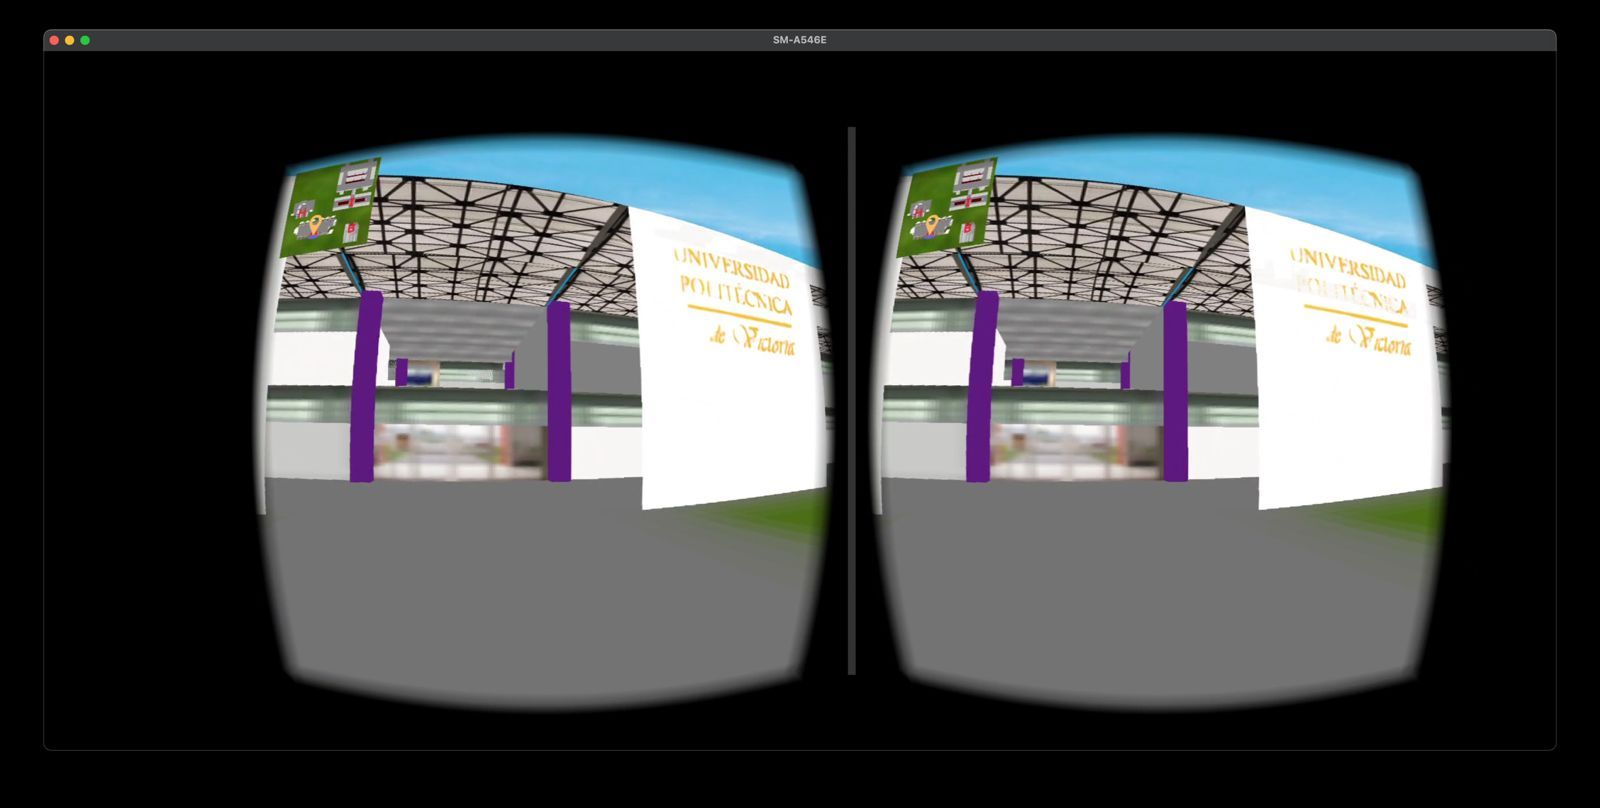
\includegraphics[width=0.8\columnwidth]{Capturas/img1.jpeg}}
        \caption{Entrada a la UPV}
        \label{fig:e1}
\end{figure}

En la figura \ref{fig:e2}, Se muestra el lobby del edificio A; específicamente, se presenta la entrada al auditorio, donde se encuentra ubicado el guardia.

\begin{figure}[h]
    \centering
        {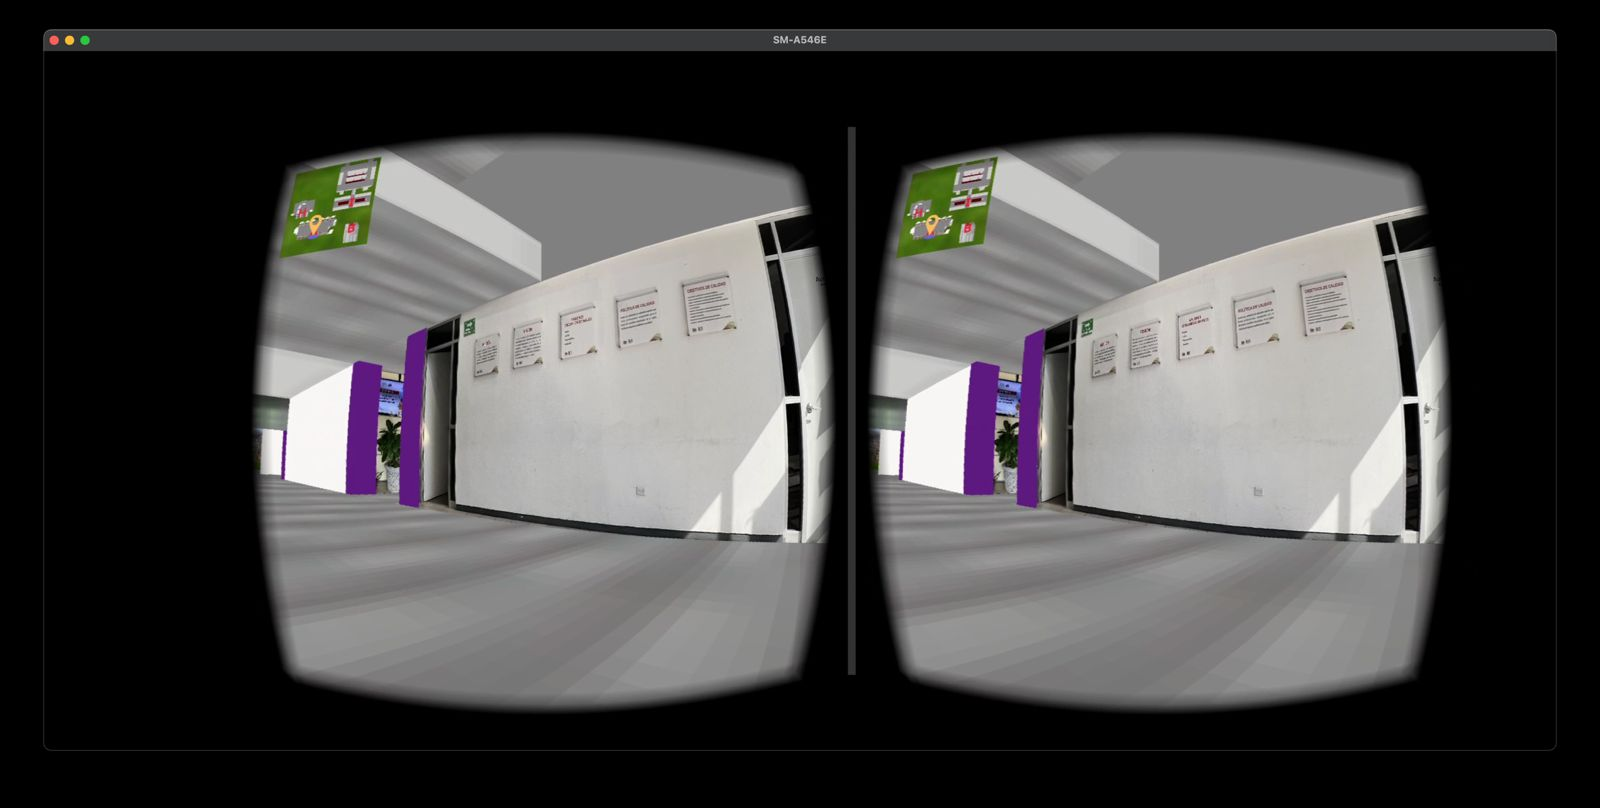
\includegraphics[width=0.8\columnwidth]{Capturas/img2.jpeg}}
        \caption{Pasillos del edificio A de la UPV (1)}
        \label{fig:e2}
\end{figure}

En la figura \ref{fig:e3}, Se muestra el lobby del edificio A, específicamente un poco más adelante de la entrada, en la zona donde se encuentra la televisión y el pasillo que conduce hacia la explanada o las escaleras que llevan al piso superior.
\begin{figure}[h]
    \centering
        {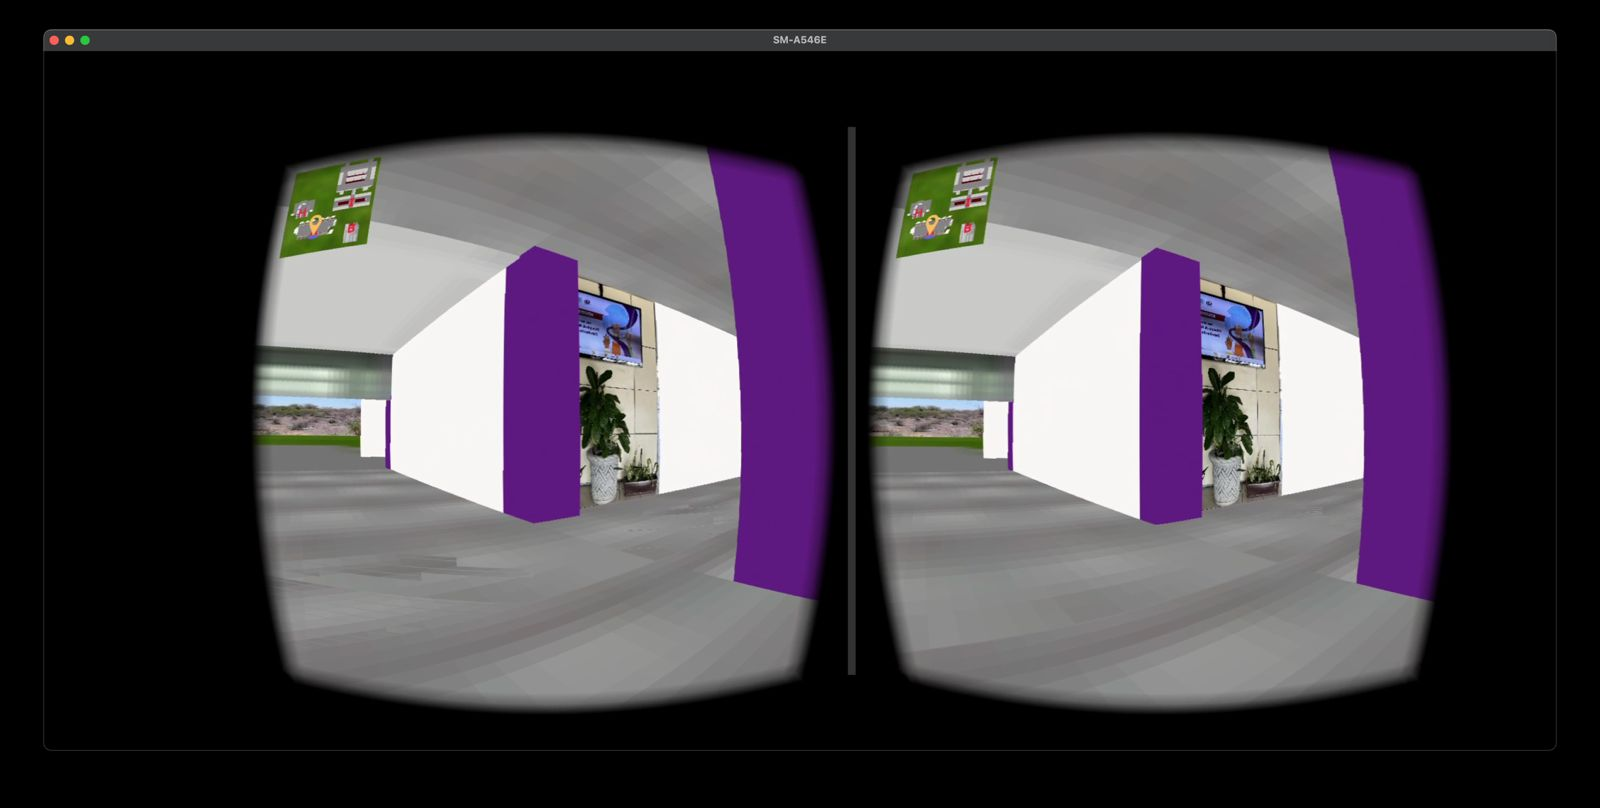
\includegraphics[width=0.8\columnwidth]{Capturas/img3.jpeg}}
        \caption{Pasillos del edificio A de la UPV (2)}
        \label{fig:e3}
\end{figure}

En la figura \ref{fig:e4}, Se presenta una vista aérea del campus de la Universidad Politécnica de Victoria (UPV).
\begin{figure}[h]
    \centering
        {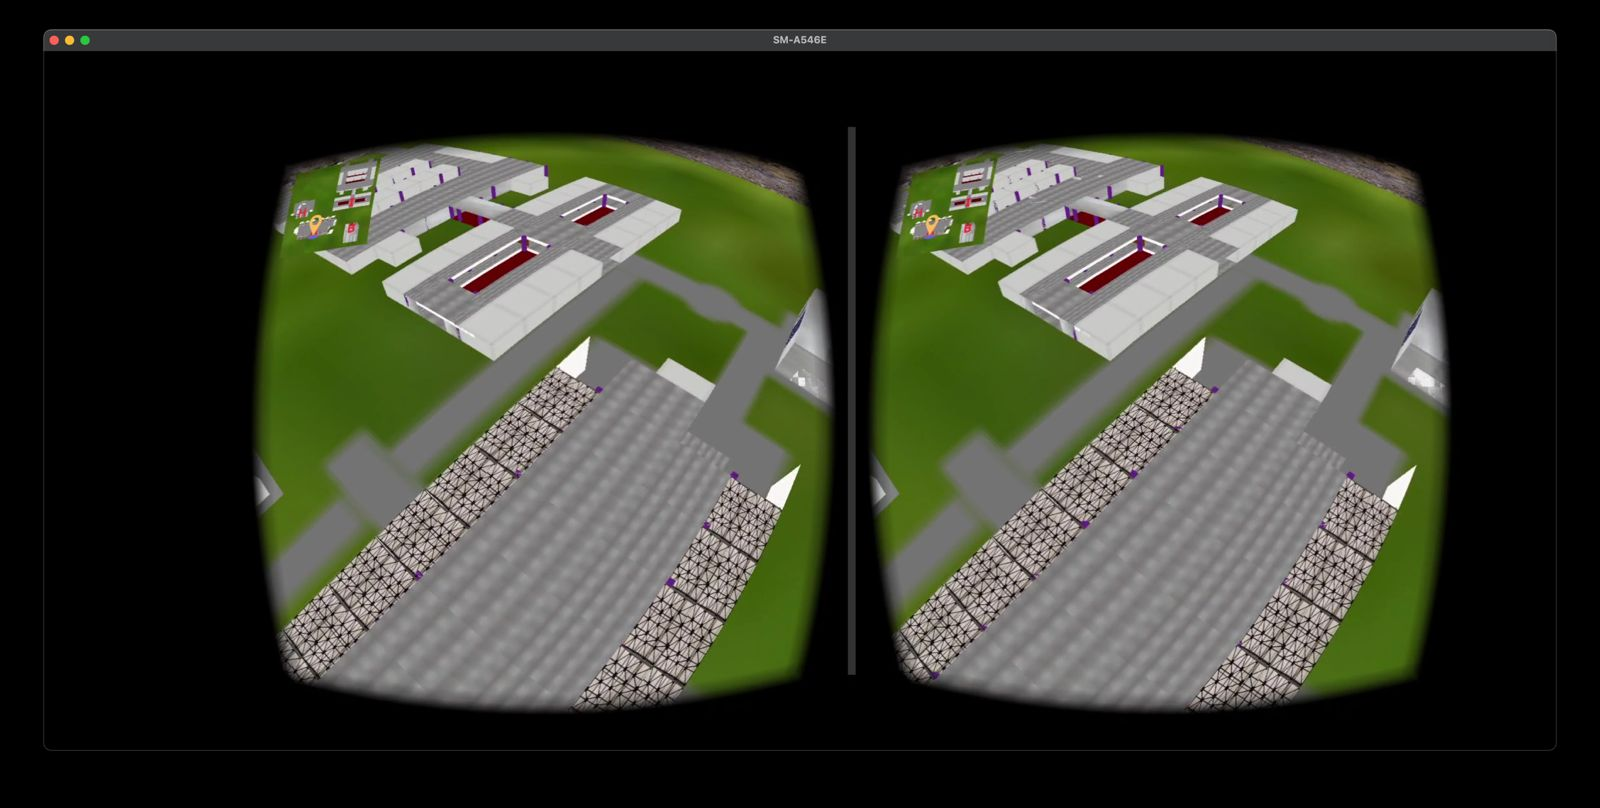
\includegraphics[width=0.8\columnwidth]{Capturas/img4.jpeg}}
        \caption{Vista aérea UPV}
        \label{fig:e4}
\end{figure}

En la figura \ref{fig:e5}, Se muestra una vista amplea de lo que es el edificio I de la Universidad Politécnica de Victoria (UPV).

\begin{figure}
    \centering
    {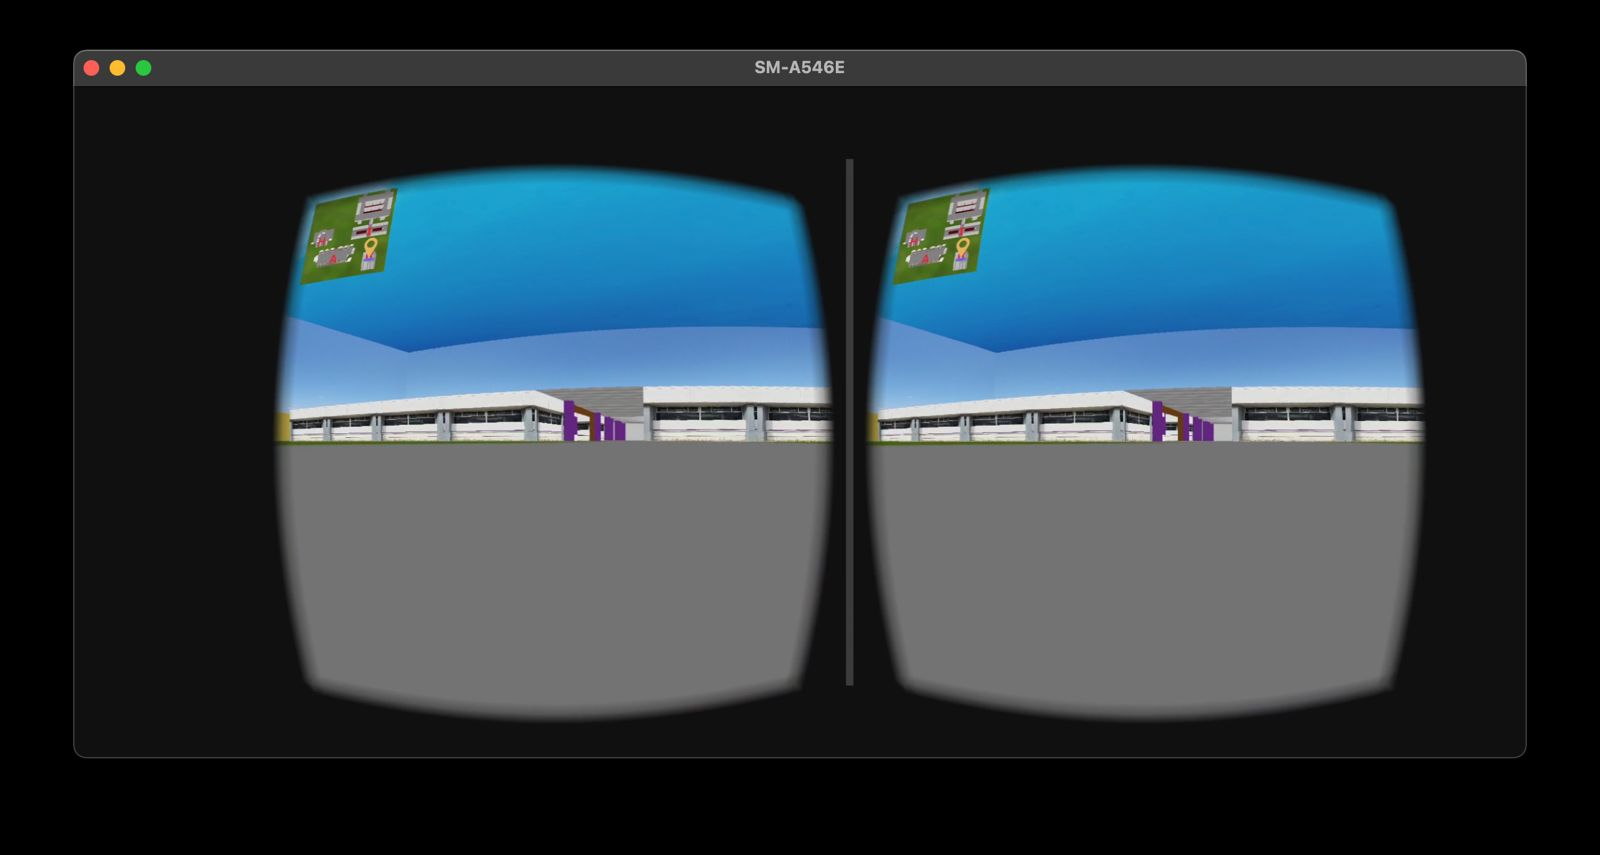
\includegraphics[width=0.8\columnwidth]{Capturas/img5.jpg}}
        \caption{Vista del edificio I}
        \label{fig:e5}
\end{figure}

\newpage

\section{Conclusión}
La aplicación desarrollada ha logrado cumplir su propósito principal de ofrecer una experiencia inmersiva y accesible para recorrer virtualmente \cite{Sh:10} las instalaciones de la Universidad Politécnica de Victoria. Al utilizar tecnologías como OpenGL \cite{Sh:4} y el Cardboard SDK, se ha creado un entorno virtual que permite a los usuarios explorar el campus con movimiento en 360° y una vista estereoscópica, generando la sensación de estar físicamente presente en la institución.

La integración del recorrido original con las nuevas funcionalidades fue un aspecto clave del desarrollo. Se respetó la estructura original, incorporando mejoras significativas como el uso de un mando de Xbox para facilitar la navegación y controles intuitivos, lo que asegura una experiencia fluida y accesible. Además, el enfoque en la precisión de la proyección de texturas y la incorporación del logo institucional refuerzan la identidad visual del proyecto.

Esta aplicación no solo facilita el acceso remoto a las instalaciones del campus, sino que también abre nuevas posibilidades para que futuros estudiantes y visitantes conozcan la universidad de manera innovadora. Los objetivos establecidos se han alcanzado de manera satisfactoria, consolidando una base sólida para el recorrido virtual. Este proyecto demuestra el potencial de las tecnologías utilizadas y establece un punto de partida para futuras expansiones que puedan enriquecer aún más la experiencia del usuario. 

\addcontentsline{toc}{section}{Referencias} 
\printbibliography
%\balance



\end{document}













